\chapter{Introduction}\label{chap:introduction}
The proposed project for this semester is a multi-project involving the entire Software 6 class. The overall purpose of the project, called GIRAF, is to create a set of applications for the Android platform, designed to help autistic people and their guardians throughout their day. Examples of this are applications like Stemmespillet, which helps people learn how loud they are, and PiktoOplæser which helps with communication by using pictograms and audio.
Previous Software 6 classes have also worked on the GIRAF multi-project, see the GIRAF multi-project logo in figure \ref{fig:GIRAFlogo}. This means that even from the beginning of the semester there was an existing code base to work on. While previous classes had developed several applications, none of them was in a state where they were ready for release. In general, most applications had crash issues and were missing a required connection to the designed database. Some applications were missing features or had implemented some bad workarounds to make it run. It was decided that the focus of this class should be to refactor and rework these programs to a degree where they could be released. Therefore, no new applications was made this semester.
The development of applications has been based on requests and feedback from customers consisting of guardians working with autistic people, primarily children. This means that at the end of the semester, the applications ideally consist of tools that both the guardians and children can use effectively.

\begin{figure}[H]
	\centering
	
\includegraphics[scale=1]{Pics/ic_giraf.png}
	\caption{The GIRAF multi-project icon.}
	\label{fig:GIRAFlogo}
\end{figure}

To give an example of the applications and their interaction with each other in the GIRAF multi-project, figure \ref{fig:sekvensContext} displays how Sekvens depends on Launcher, GUI, and OasisLib, and utilizes Sequenceviewer, and PictoSearch.
\begin{figure}[H]
	\centering
	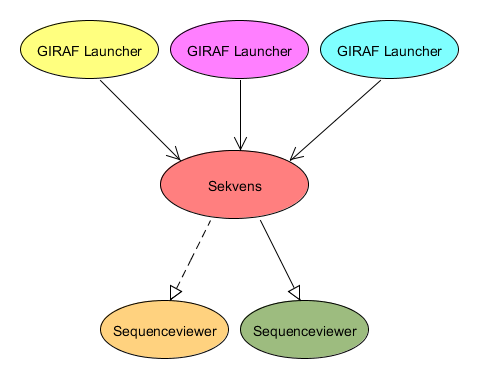
\includegraphics[scale=0.4]{Pics/sekvens.png}
	\caption{The position of Sekvens in the multi-project after Sprint 4.}
	\label{fig:sekvensContext}
\end{figure}
